%class
\documentclass[a4paper, 12pt]{article}

%encoding
\usepackage[T1]{fontenc}           %font encoding
\usepackage[utf8]{inputenc}         %script encoding

%packages
\usepackage[czech]{babel}           %language
\usepackage[a4paper, text={17cm,24cm}, left=2cm, top=3 cm]{geometry}		%layout
\usepackage[unicode,hidelinks]{hyperref}	%links
\usepackage{amsmath}
\usepackage[bottom]{footmisc}
\usepackage{tabularx}
\usepackage{graphicx}
\usepackage{float}
\usepackage{csquotes}

\usepackage[backend=biber,style=iso-numeric,bibencoding=UTF8]{biblatex}
\addbibresource{sources.bib}

\begin{document}
	
	\begin{titlepage}
		\centering
		
		
\includegraphics{src/fitlogo.pdf}
		
		\vspace{\stretch{0.382}}
		
		{\Huge Protokol k projektu z ISS\\[0.4em]
			\LARGE David Tobolík (xtobol06)}
		
		\vspace{\stretch{0.618}}
	\end{titlepage}
	
	\tableofcontents
	\newpage
	
	\section{Základy}
	Na obrázku~\ref{fig:signaly} můžeme vidět 3 signály a jejich spektra, spočítané pomocí FFT\footnote{Fast Fourier Transform -- konkrétně jeho implementace v knihovně numpy\cite{np} jazyka Python}, která vychází z DFT~(Discrete Fourier Transform) \cite{DFT} popsané v rovnici \eqref{DFT}. Tón MIDI 29 v sobě má mnohem více nepravidelností, které se ukazují i ve spektru. Zatímco tóny s vyšší frekvencí jsou pravidelnější a i jejich spektrum má výrazněji oddělené násobky základní frekvence, to hraje důležitou roli v následujících úkolech.
	
	\begin{equation}
		X_k = \sum_{n=0}^{N-1} x_n e^{- \frac{2 \pi i}{N}} n k \qquad k = 0, \dots, N-1 \label{DFT}
	\end{equation}

	\begin{figure}[H]
		\begin{minipage}{.5\textwidth}
			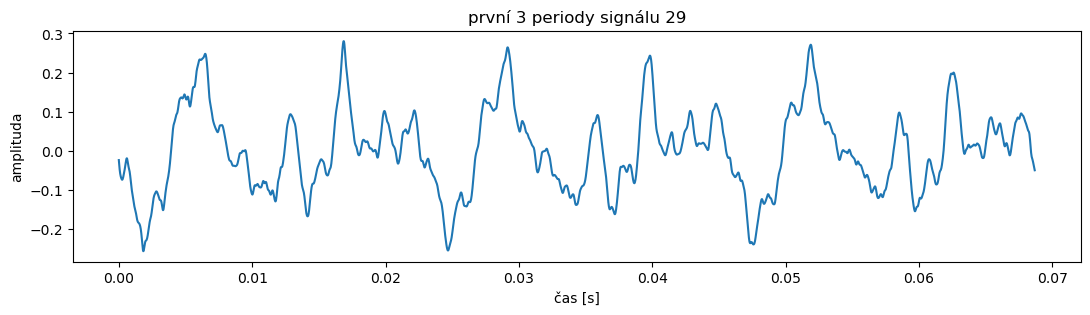
\includegraphics[width=\textwidth]{src/sign_a.png}
		\end{minipage}
		\begin{minipage}{.5\textwidth}
			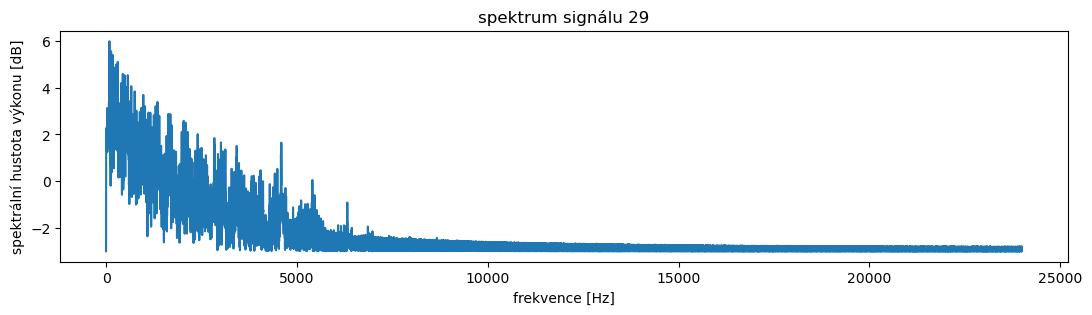
\includegraphics[width=\textwidth]{src/spectr_a.png}
		\end{minipage}
		
		\begin{minipage}{.5\textwidth}
			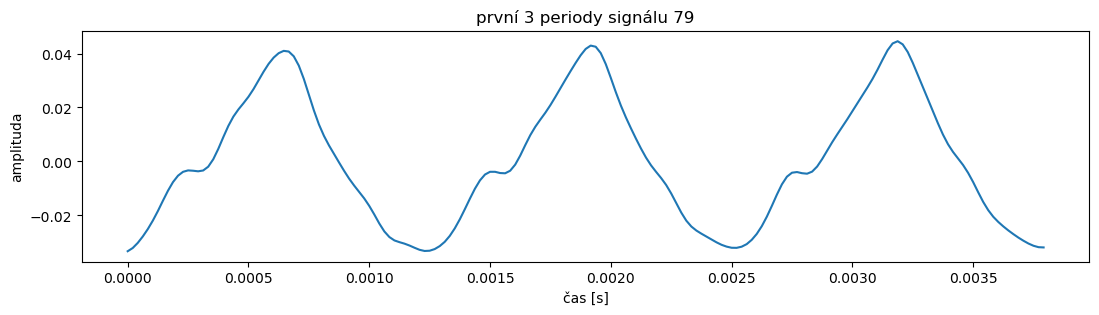
\includegraphics[width=\textwidth]{src/sign_b.png}
		\end{minipage}
		\begin{minipage}{.5\textwidth}
			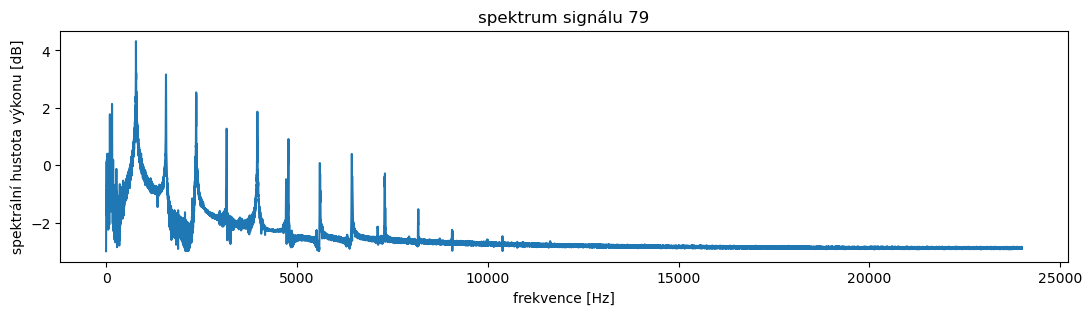
\includegraphics[width=\textwidth]{src/spectr_b.png}
		\end{minipage}
		
		\begin{minipage}{.5\textwidth}
			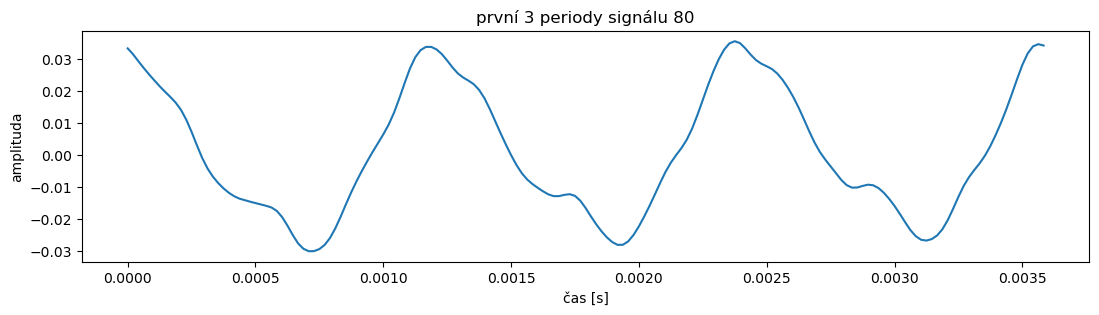
\includegraphics[width=\textwidth]{src/sign_c.png}
		\end{minipage}
		\begin{minipage}{.5\textwidth}
			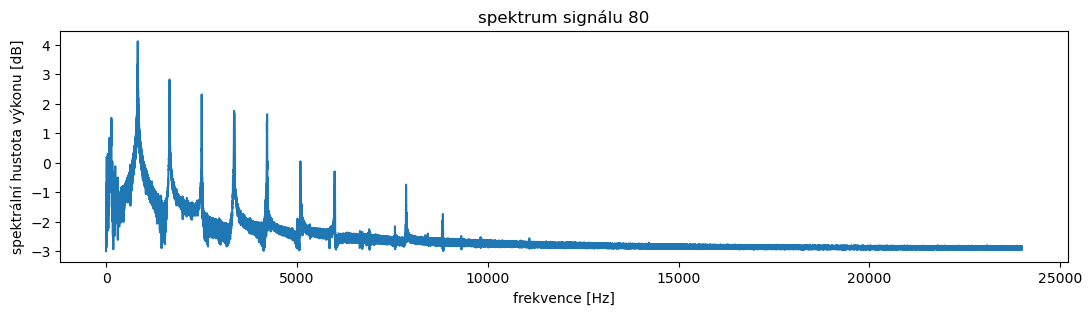
\includegraphics[width=\textwidth]{src/spectr_c.png}
		\end{minipage}
		\caption{Přidělené signály a jejich spektra}
		\label{fig:signaly}
	\end{figure}

	\pagebreak
	\section{Určení základní frekvence}
	Základní frekvence byla určena pomocí autokorelace \eqref{korel} a to zvlášť pro nižší a vyšší frekvence (interval byl rozdělen na polovinu). Pro nižší frekvence byl nalezen 10. největší\footnote{číslo 10 bylo zvoleno po experimentálním měření} koeficient, jehož x-ová pozice byla vydělena 10, tím se získala průměrná vzdálenost vrcholů, tedy průměrná vzdálenost opakování základní frekvence signálu. Tato metoda byla zvolena především proto, že u krajních korelačních koeficientů nižších frekvencí není tak znatelný rozdíl a mohou se překrývat, což je způsobeno malým překryvem signálu při výpočtu autokorelace a tím způsobenou nepřesností, proto byly měřeny první vrcholy, které jsou dostatečně odlišitelné.
	
	Naopak u tónu s vyšší frekvencí je tato metoda nepřesná, protože vrcholy jsou blízko u sebe a proto průměr není tak přesný. Zato jsou vrcholy dobře rozlišitelné od sebe, to tedy znamená, že lze vzít více vrcholů, které následně zprůměrujeme. Experimentálně bylo určeno, že pro vyšší frekvence jsou všechny vrcholy dostatečně odlišitelné. Vzdálenost prvního a posledního vrcholu $\Delta n \simeq N$, kde $N$ je počet korelačních koeficientů, lze tedy říct, že $\frac{k\Delta n}{N} \simeq k$, kde $k$ je počet vrcholů.
	
	\begin{equation}
		R_{xx}[k] = \frac{1}{N} \sum_{n = 0}^{N - 1} x[n]x[n + k] \label{korel}
	\end{equation}

	\begin{figure}[H]
		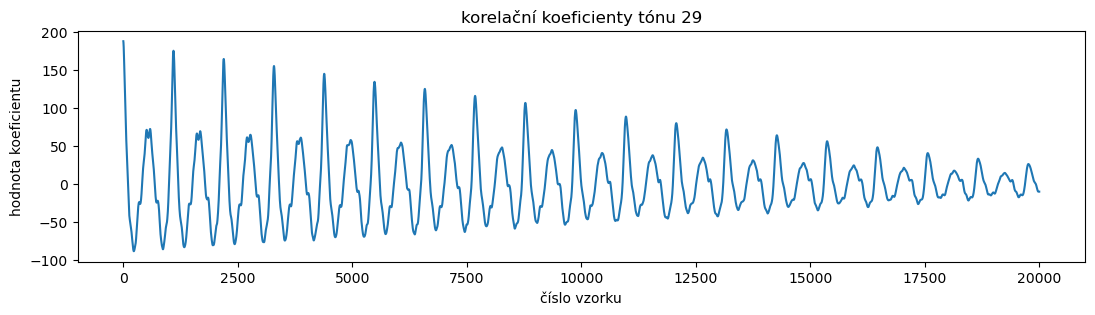
\includegraphics[width=\textwidth]{src/corel_a.png}
		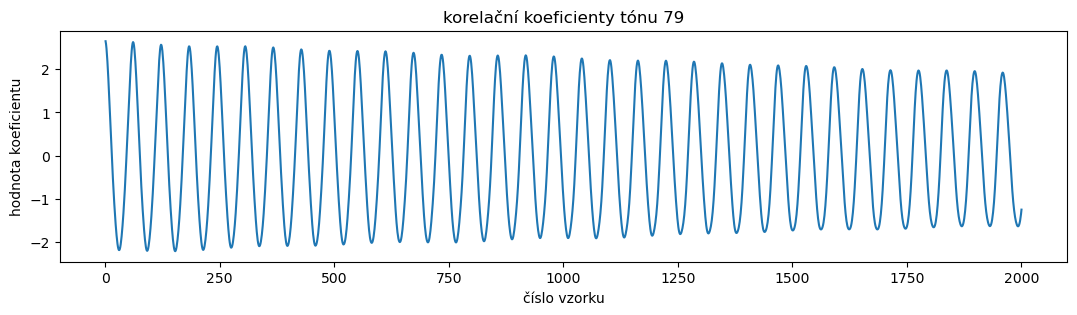
\includegraphics[width=\textwidth]{src/corel_b.png}
		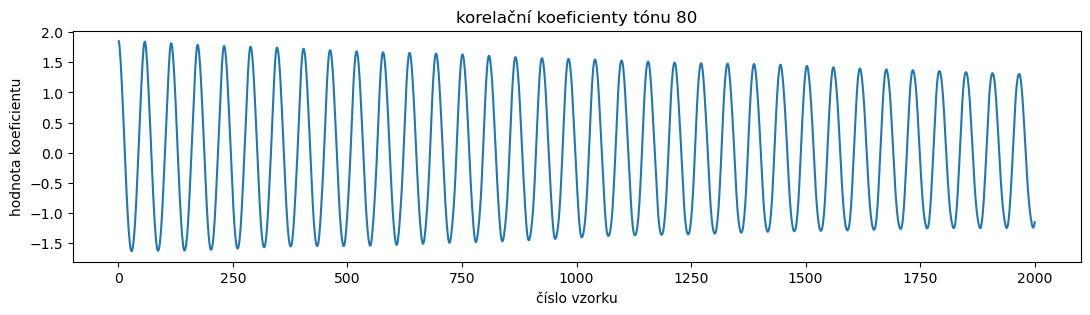
\includegraphics[width=\textwidth]{src/corel_c.png}
		\caption{prvních 2000 autokorelačních koeficientů přidělených signálů}
	\end{figure}

	\subsection{Odhadnuté hodnoty základních frekvencí}
	\begin{table}[H]
		\begin{tabularx}{\textwidth}{r|Xr|Xr|Xr|X}
		MIDI & $f_0 [Hz]$ &        MIDI & $f_0 [Hz]$  &        MIDI & $f_0 [Hz]$ & MIDI & $f_0 [Hz]$ \\ \hline
		24 & 32.78        &        46 & 116.98        &        68 & 419.0 &        90 & 1479.0 \\
		25 & 34.72        &        47 & 124.03        &        69 & 443.0 &        91 & 1567.0 \\
		26 & 36.79        &        48 & 131.50        &        70 & 471.0 &        92 & 1661.0 \\
		27 & 38.97        &        49 & 139.13        &        71 & 495.0 &        93 & 1759.0 \\
		28 & 41.28        &        50 & 146.92        &        72 & 523.0 &        94 & 1865.0 \\
		29 & 43.73        &        51 & 155.64        &        73 & 555.0 &        95 & 1977.0 \\
		30 & 46.33        &        52 & 164.89        &        74 & 587.0 &        96 & 2095.0 \\
		31 & 49.08        &        53 & 176.47        &        75 & 623.0 &        97 & 2219.0 \\
		32 & 51.99        &        54 & 186.04        &        76 & 659.0 &        98 & 2351.0 \\
		33 & 55.08        &        55 & 198.34        &        77 & 699.0 &        99 & 2491.0 \\
		34 & 58.35        &        56 & 210.52        &        78 & 739.0 &        100 & 2639.0 \\
		35 & 62.17        &        57 & 222.22        &        79 & 783.0 &        101 & 2793.0 \\
		36 & 65.75        &        58 & 235.29        &        80 & 831.0 &        102 & 2961.0 \\
		37 & 69.76        &        59 & 250.0         &        81 & 879.0 &        103 & 3137.0 \\
		38 & 73.47        &        60 & 266.66        &        82 & 931.0 &        104 & 3325.0 \\
		39 & 77.84        &        61 & 282.35        &        83 & 989.0 &        105 & 3521.0 \\
		40 & 82.47        &        62 & 296.29        &        84 & 1047.0&        106 & 3731.0 \\
		41 & 87.65        &        63 & 311.68        &        85 & 1109.0&        107 & 3953.0 \\
		42 & 92.87        &        64 & 333.33        &        86 & 1175.0&        108 & 4189.0 \\
		43 & 98.40        &        65 & 352.94        &        87 & 1245.0& & \\
		44 & 104.23       &        66 & 371.0         &        88 & 1319.0& & \\
		45 & 110.42       &        67 & 391.0         &        89 & 1397.0& & \\
		\end{tabularx}
	\caption{Tabulka základních frekvencí odhadnutých z koeficientů autokorelace}
	\end{table}
	
	\pagebreak
	\section{Zpřesnění odhadu základní frekvence} \label{dtft}
	Byla použita metoda DTFT (Discrete Time Fourier Transform) s rozsahem 5 Hz na každou stranu od odhadnuté frekvence. V tomto okolí bylo nalezeno maximum, které považujeme za základní frekvenci. Pro tóny s nízkou frekvencí bylo hledáno maximum na dvojnásobku odhadnuté základní frekvence a hodnota následně vydělena 2.
	
	\begin{figure}[H]
		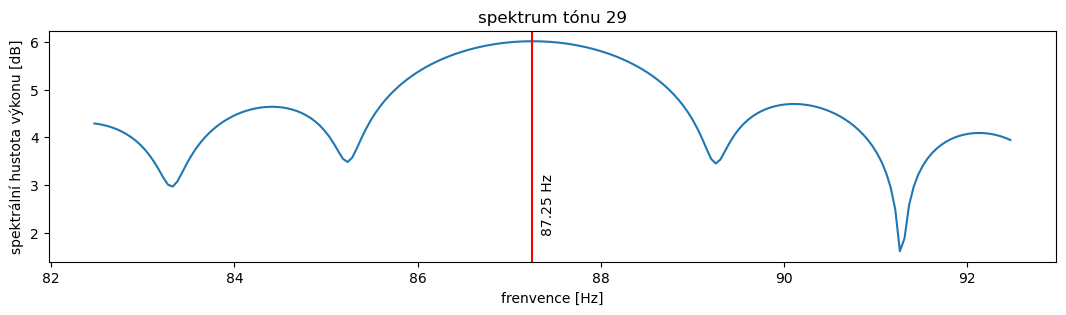
\includegraphics[width=\textwidth]{src/prec_a.png}
		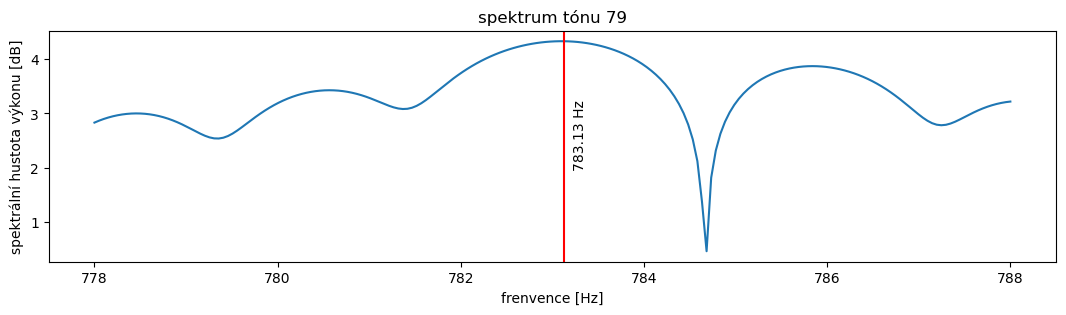
\includegraphics[width=\textwidth]{src/prec_b.png}
		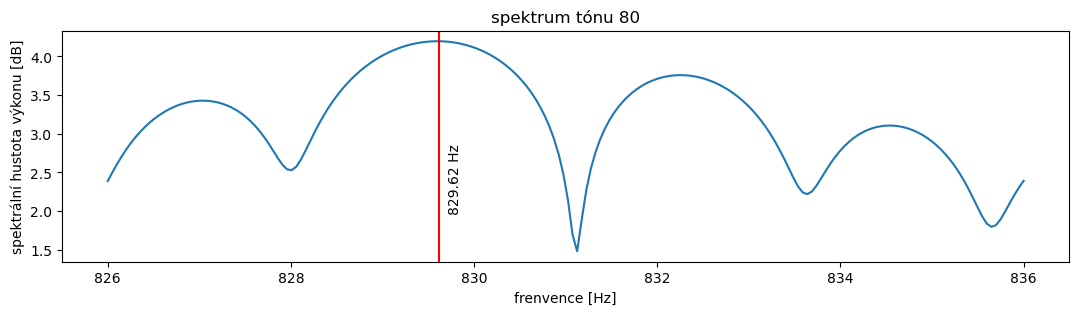
\includegraphics[width=\textwidth]{src/prec_c.png}
		\caption{Spektrum okolí odhadnuté základní frekvence si vyznačeným maximem}
	\end{figure}

	\subsection{Výsledné hodnoty základních frekvencí}
	Dále je počítáno s těmito hodnotami, i přes občasné odchylky jsou ve výsledku přesnější než odhadnuté hodnoty. Odchylky mohou být způsobeny jak špatným naladěním piana, tak časovým intervalem, který je analyzován. Především v nízkých frekvencích po určité době začnou zanikat některé složky a v signálu se vytváří nepravidelnosti.
	
	\begin{table}[H]
		\begin{tabularx}{\textwidth}{r|Xr|Xr|Xr|X}
			MIDI & $f_0 [Hz]$ &        MIDI & $f_0 [Hz]$  &        MIDI & $f_0 [Hz]$ & MIDI & $f_0 [Hz]$ \\ \hline
			24 & 32.66     &       46 & 116.57     &       68 & 415.45     &       90 & 1478.92 \\
			25 & 34.61     &       47 & 123.18     &       69 & 440.11     &       91 & 1566.92 \\
			26 & 36.67     &       48 & 130.43     &       70 & 466.25     &       92 & 1660.07 \\
			27 & 38.86     &       49 & 138.16     &       71 & 493.81     &       93 & 1758.92 \\
			28 & 41.17     &       50 & 147.08     &       72 & 523.17     &       94 & 1863.61 \\
			29 & 43.62     &       51 & 155.88     &       73 & 554.27     &       95 & 1976.47 \\
			30 & 46.21     &       52 & 165.18     &       74 & 587.17     &       96 & 2093.96 \\
			31 & 48.97     &       53 & 174.77     &       75 & 622.12     &       97 & 2218.52 \\
			32 & 51.88     &       54 & 185.15     &       76 & 659.07     &       98 & 2350.67 \\
			33 & 54.97     &       55 & 196.17     &       77 & 697.56     &       99 & 2490.42 \\
			34 & 58.22     &       56 & 208.12     &       78 & 739.07     &       100 & 2638.52 \\
			35 & 61.66     &       57 & 220.50     &       79 & 783.12     &       101 & 2795.08 \\
			36 & 65.31     &       58 & 233.59     &       80 & 829.61     &       102 & 2961.22 \\
			37 & 69.20     &       59 & 247.50     &       81 & 878.97     &       103 & 3137.37 \\
			38 & 73.43     &       60 & 264.59     &       82 & 931.32     &       104 & 3324.02 \\
			39 & 77.80     &       61 & 280.17     &       83 & 987.61     &       105 & 3521.67 \\
			40 & 82.41     &       62 & 293.79     &       84 & 1046.17    &       106 & 3731.12 \\
			41 & 87.34     &       63 & 310.84     &       85 & 1108.32    &       107 & 3953.17 \\
			42 & 92.54     &       64 & 330.83     &       86 & 1174.22    &       108 & 4188.27 \\
			43 & 98.03     &       65 & 350.64     &       87 & 1244.12    & & \\
			44 & 103.87    &       66 & 370.03     &       88 & 1318.17    & & \\
			45 & 110.03    &       67 & 391.87     &       89 & 1395.91    & & \\
		\end{tabularx}
	\caption{Tabulka základních frekvencí určených DTFT}
	\end{table}
	
	\section{Reprezentace klavíru}
	Každý tón jsem se rozhodl reprezentovat 5 komplexními čísly a to prvními 5 koeficienty DTFT základní frekvence daného tónu. Pro každý tón byl proveden výpočet násobku základní frekvence z maxima v okolí (stejně jako v \ref{dtft}) a byl uložen prvek DTFT, na který toto maximum připadalo.
	
	U tónu MIDI 79 můžeme vidět vychýlení od maxim ve spektru. To může být způsobeno nepřesností FFT nebo rozladěním piana. 5. maximum by určitě mělo být okolo $f_0 * 5 = 783.12 * 5 = 3915.6$, ale je až okolo $4100$. Rozhodl jsem se, ale držet základní frekvence (které jsou celkem přesné), aby nedošlo ke zkreslení tónů.
	
	U nízkých frekvencí můžeme opět vidět značné nepřesnosti, které mají vliv i na vypočítaná maxima.
	
	\begin{figure}[H]
		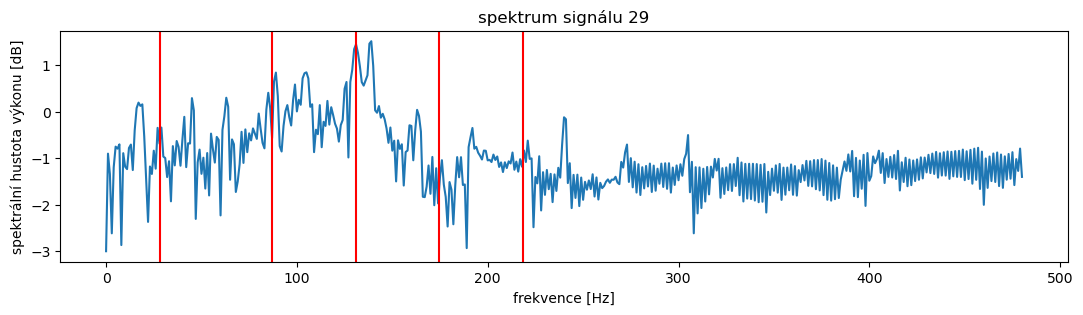
\includegraphics[width=\textwidth]{src/base_a.png}
		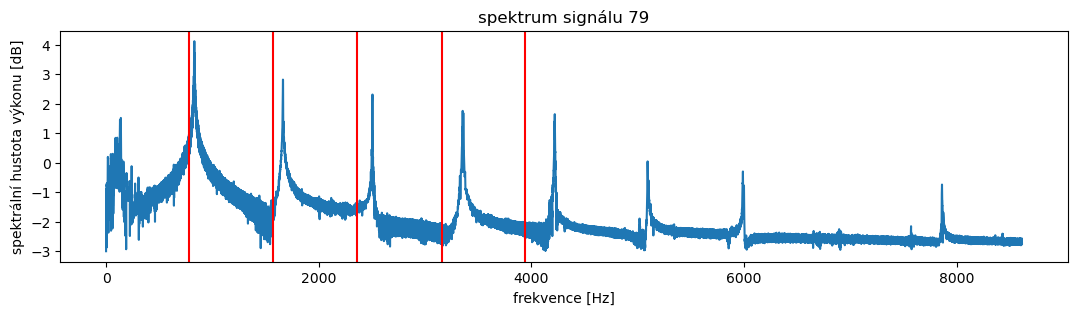
\includegraphics[width=\textwidth]{src/base_b.png}
		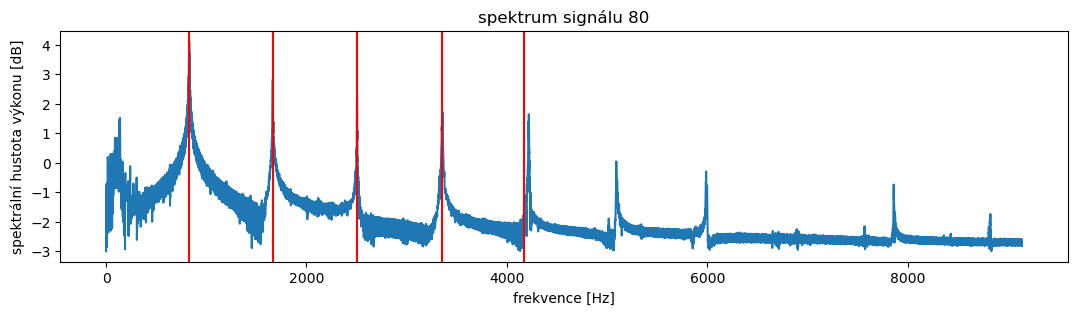
\includegraphics[width=\textwidth]{src/base_c.png}
		\caption{Nalezená maxima násobků základních frekvencí (spektrum je vypočítané FFT)}
	\end{figure}
	
	\section{Syntéza tónů}
	Tóny byly syntetizovány zpětnou transformací pomocí Fourierovy řady. Pro každé z 5 komplexních čísel byl přičten příslušný sinus a cosinus vynásobený po řadě imaginární a reálnou složkou a to pro každé $n$ v generovaném signálu.
	
	Reprezentace signálu neumožňuje práci s dynamikou tónu, takže všechny tóny jsou konstantní a neodráží barevnost původní nahrávky. Vidíme, že došlo k určitému vyhlazení a ztrátě informace, způsobené malým paměťovým prostorem, na kterém je každý signál uložen.
	
	$$ a_k[n] = x_{im} sin(2 \pi \frac{k}{N} n) \qquad k = f_0, \dots, 5f_0$$
	$$ b_k[n] = x_{re} cos(2 \pi \frac{k}{N} n) \qquad k = f_0, \dots, 5f_0$$
	
	\begin{figure}[H]
		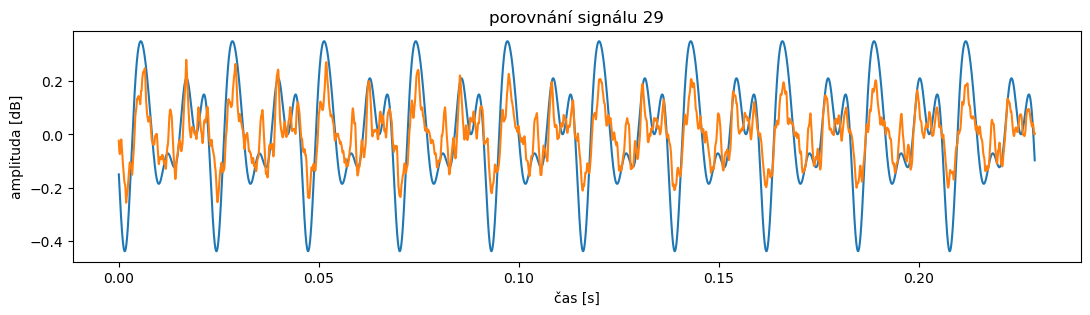
\includegraphics[width=\textwidth]{src/synth_a.png}
		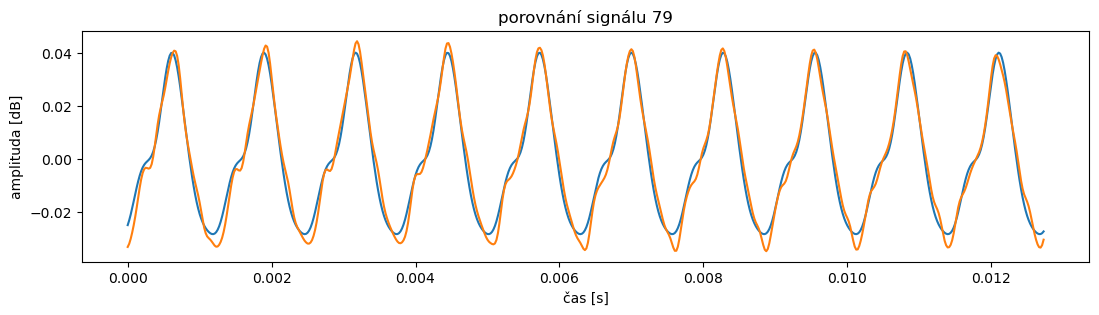
\includegraphics[width=\textwidth]{src/synth_b.png}
		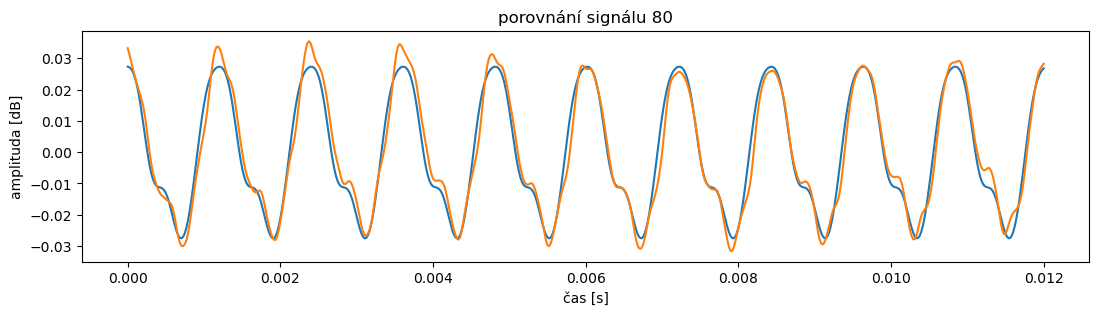
\includegraphics[width=\textwidth]{src/synth_c.png}
		\caption{Porovnání syntetizovaného signálu (modrá) s původní nahrávkou (oranžová)}
	\end{figure}
	
	\section{Generování hudby}
	Generování hudby probíhalo stejně jako generování jednotlivých tónů, navíc se ještě vynásobil generovaný signál hlasitostí tónu.
	
	Ve skladbě (především se vzorkovací frekvencí 48 kHz) lze slyšet praskání, které je způsobené náhlým oříznutím signálu. Toto by šlo vylepšit postupným snižováním hlasitosti před koncem znění tónu nebo prolnutí s dalším tónem.
	
	Díky tomu, že vygenerované tóny postrádají dynamiku, zní skladba jako kdyby byla hrána spíše na varhany, u kterých se klapka v píšťalách otevře a zavře velmi rychle, na rozdíl od piana, kde struna zní ještě dlouho a pomalu utichá.
	
	\section{Spektrogram}
	Na spektrogramech jednotlivých nahrávek můžeme vidět, že jsou nejvíce zastoupeny frekvence do 2000 Hz, zde se totiž nachází většina základních frekvencí a i jejich násobky (resp. prvních 5, které používáme). Vzorkovací frekvence 48 kHz je tedy v tomto případě zbytečně velká, protože nemůže být rozumně využita. Nejvyšší frekvence, kterou dokážeme vygenerovat je mírně pod 21 kHz, ale toto je hodnota pro MIDI 108. Ve skladbě je nejvyšší tón MIDI 86, u kterého se generuje maximální frekvence někde okolo 5900 Hz.
	
	Svislé čáry ve spektrogramu jsou ono zmíněné lupání, nachází se na přelomu tónů (všimněme si jejich hustoty okolo 3. sekundy a poslechněme si skladbu v tomto čase).
	
	Mimo jiné na spektrogramu vidíme pěkně násobky základních frekvencí hraných tónů a jejich hlasitost. Nejnižší frekvence mají nejvyšší energii, což se shoduje s tím, co vidíme na spektru na obrázku \ref{fig:signaly}.
	
	\begin{figure}[H]
		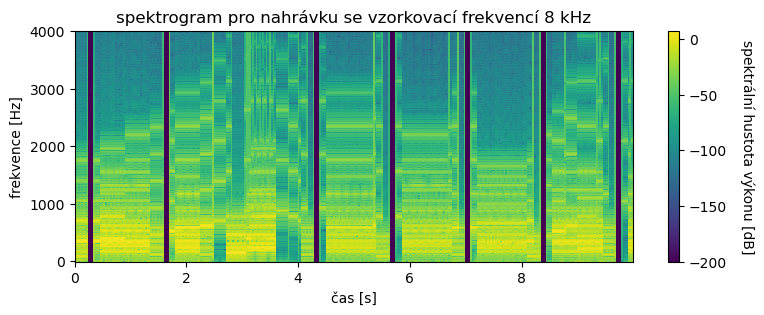
\includegraphics[width=\textwidth]{src/spectr_8k.png}
		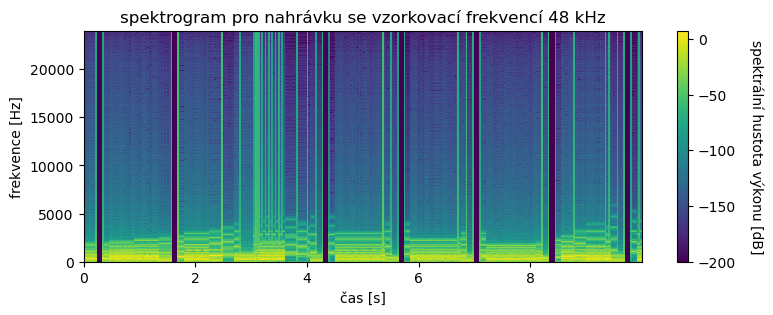
\includegraphics[width=\textwidth]{src/spectr_48k.png}
		\caption{Spektrogramy pro vygenerované nahrávky}
	\end{figure}
	
	\newpage
	%bibliography
	\renewcommand{\refname}{Zdroje}
	\printbibliography
\end{document}
